\documentclass[a4paper, 11pt]{article}
\usepackage[margin=1in]{geometry}
\usepackage{multirow}
\usepackage{amsmath}
\usepackage{amssymb}
\usepackage{graphicx}
\usepackage{float}
\usepackage{parskip}
\usepackage{enumitem}
\usepackage{graphicx}
\usepackage{caption}
\usepackage{subcaption}
\usepackage{tikz}
\usepackage{courier} 
\usepackage{listings}
\usepackage{minted}
\usepackage{subfig}
\usepackage{qtree}\usepackage{makecell}
\usepackage{float}
\usepackage{url}
\usepackage{hyperref}
\usepackage[colorlinks=true, allcolors=blue]{hyperref}
\usepackage{longtable}
\usepackage{xcolor}
\usepackage{tabularx}
\lstset{                    % Code langugage
basicstyle=\ttfamily,   
}
\title{Workshop 1: 4-bit CPU Design}
\author{Charles Khoury \\
\href{mailto:ck15960@my.bristol.ac.uk}{charles.khoury@bristol.ac.uk}}

\begin{document}
\maketitle

\section{Introduction}

The goal of this workshop is to gain a better understanding of the inner-workings of the 4-bit CPU and understand the design philosophy. The CPU is designed using ModuleSim which simulates hardware previously used in the delivery of the introductory unit to computer architecture for undergraduates, the modules were meant to work in tandem with the simulation; hence the unusual component choice. This implies the need to work around the design constrains set by the design tool.

\section{Basic design knowledge}
Fundamentally CPUs are Finite State Machines (FSM) containing the following component block:
\begin{itemize}
  \item Control Unit (CU).
  \item Arithmetic Logic Unit (ALU).
  \item Registers.
  \item Buses (internal data lines).
  \item Clock
  \item Cache
\end{itemize}
The processor in this unit doesn't have a cache, instead instructions are fetched directly from memory (NRAM component in ModuleSim).\\
\textbf{ALU}: performs arithmetic and logical operation and in for the 4-bit processor the part of the multistage memory write process (see STAM). \\
\textbf{CU}: Performs the Fetch, Decode, Execute operations by issuing control  signals to the hardware and moving data around.\\
\textbf{Registers}: Small amount of memory contained within the CPU to store data needed to perform the various functions. Such as instruction address, current opcode and optional operand, result of calculations. Modern processors possess specific function registers (such as the Program Counter (PC), Instruction Register, etc.) and general purpose register than can be used to store addresses, computation results etc. \\
\textbf{Clock}: Used to synchronize the different CPU components. \\
This computational model is what is know as the Von Neumann architecture. 

\begin{figure}[H]
    \centering
    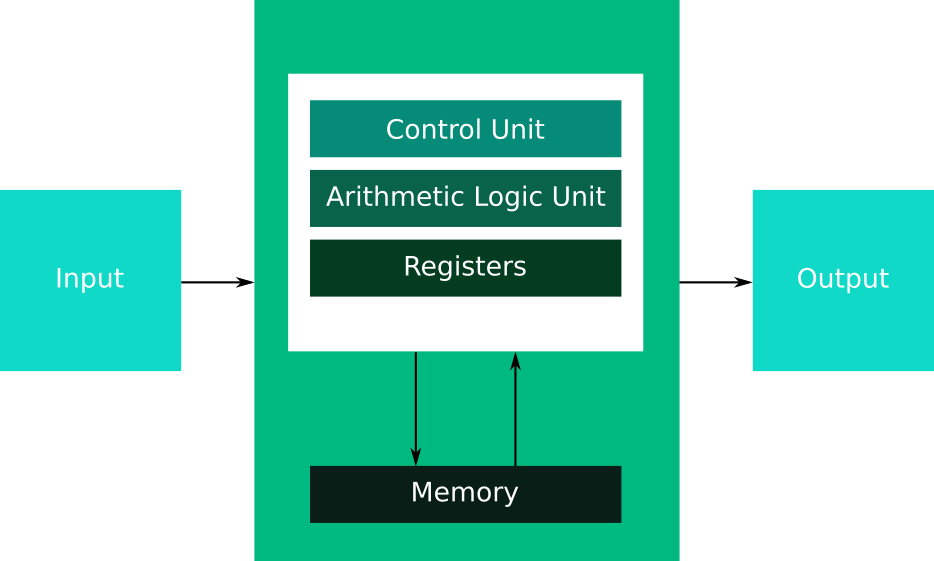
\includegraphics[width =0.57\textwidth]{Images/von-neuman-arch.png}
    \caption{Von Neumann Architecture diagram}
    \label{fig:vn-arch}
\end{figure}

\section{Understanding the Instruction Set}
\subsection{Instruction Set Architecture}
The base implementation of the 4-bit uses 8 instructions encoded over 4 bits. \\
\textbf{Question:} Theoretically, how many instructions can be encoded over 4 bits? \\
\begin{table}[H]
\centering
\begin{tabularx}{\textwidth}{|l c X|}
  \hline

  Mnemonic & Operands/Example & Description \\
  \hline

\verb|LDAC| & \textit{Cn} & Load constant in register A \\
& \verb|LDAC 5| & Load 5 into register A\\
  \hline
  \verb|LDBC| & \textit{Cn} & Load constant in register B \\
& \verb|LDBC 5| & Load 5 into register B\\
  \hline
  \verb|LDAM| & \textit{Addr} & Load LSB at address of \textit{Addr} into register A \\
& \verb|LDAM 10| & Load LSBs stored in memory location 10 into register A\\
  \hline
    \verb|LDBM| & \textit{Addr} & Load LSBs at address of \textit{Addr} into register B \\
& \verb|LDBM 10| & Load LSBs stored in memory location 10 into register B\\
  \hline
  \verb|STAM| & \textit{Addr} & Store the content register A in memory location \textit{Addr} and reset the MSB\\
& \verb|STAM 10| & Store content of A\\
\hline
  \verb|ADD| &  & Add the values stored in register A and B and store the result in A\\
& \verb|ADD| \textit{A = 6, B=4}, & Value of A after Phase 3b : 10\\
\hline
  \verb|SUB| &  & Substract the values stored in register A and B and store the result in A\\
& \verb|SUB| \textit{A = 6, B=4}, & Value of A after Phase 3b : 2\\
\hline
  \verb|LDAI| & \textit{offset} & Load the content from memory at address [A+offset] into A\\
& \verb|LDAI| LDAI 4 \textit{A=6,Mem10 = 12} & Load 12 into register A\\
\hline
\end{tabularx}
 \caption{4-bit CPU ISA}
 \label{Table-3}
 \end{table} 
 
\subsection{Exercise}

\textbf{Question:} What is the value stored in register B after complete execution of the following code:
\begin{lstlisting}
    LDAC 2
    LDBC 3
    ADD
    STAM 10
    LDBC 4
    SUB
    LDBM 10
\end{lstlisting}
\textcolor{red}{\textbf{Answer:}} The value in register B since the result of A+B (A=2, B=3) is stored in address 10 which is then loaded in register B in the final instruction\\
\textbf{Question:} Consider the code below:
\begin{lstlisting}
    LDAC 4
    LDBC 3
    STAM 3
    ADD
\end{lstlisting}
What is the value of register A after complete execution of this code.\\
\textcolor{red}{\textbf{Answer:}} The final value is 4 and NOT 7 as the STAM instruction overwrites the content at location 0x03 which is where the ADD instruction is located in this code.\\
\textbf{Note:} Try to understand how writing to memory affected code execution.\\
\textbf{Question:} Which instruction(s) write to Register A?\\
\textcolor{red}{\textbf{Answer:}} LDAC, LDAI, LDAM, ADD, SUB\\
\textbf{Question:} Which instruction(s) read and write to/from the main memory ?\\
\textcolor{red}{\textbf{Answer:}} LDBM, LDAI, LDAM, STAM, \\
\section{Design Implementation}
\subsection{Arithmetic Logic Unit}
\subsection{Control Unit}
As mentioned above the role of the CU is to perform the the Fetch, Decode, Execute operation by deriving control signals. \\
\textbf{Question:} What are the different entit(y/ies) that need to be controlled in the data path for each instruction ? \\ 
Derive the control signal needed for each instructions to the different components of the data path. Include a fetch and decode phase as part of your work. \\
\textcolor{red}{\textbf{Answer:}} Please refer to the file \textit{ISA\_control.pdf} \\
For this processor the CU is implemented in two part, a phase generator and decoder unit. The former allows to select the function (Fetch, Increment, [Decode-Execute]) and the latter allows you generate a control signal based on the instruction (i.e. Decode).

\subsubsection{Clock Phases}
The segmentation of the Fetch, Increment PC and [Decode-Execute] is done using the two phase clock and a counter to generate an upper phase.
The main clock has 2 non-overlapping phases $(a,b)$. 
\begin{figure}[H]
    \centering
    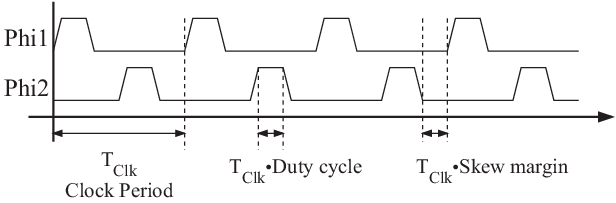
\includegraphics[width =0.57\textwidth]{Images/The-non-overlapping-two-phase-clocking-scheme.png}
    \caption{Non overlapping clock}
    \label{fig:nonoverclk}
    \end{figure}
In ModuleSim, when connected to a register the clock module is able to generate the control signal to the register as to write or reset it. From there, a counter tied to phase $b$ is used to generate a numbered phased $(1,2,3)$ (The counter can generate more phases which remain unused). \\
\textbf{Question:} By combining numbered and lettered phases, how many phases can be generated ? \\

\subsubsection{Instruction Decoding}
The decoding process determines what instruction is to be performed and produces a sequence on each control line top implement functionality. This is typically done using a binary encoder that "1-hot" encodes the signal. For the processor studied in this unit this is achieved using multiple demultiplexers. \\
\textbf{Question:} Why do we need multiple demultiplexers ? \\
\textcolor{red}{\textbf{Answer:}} The DMX module is a 2-4 demux with a 2 bit control signal (each lane represents a 4 bit bus). Since we need to implement more than 4 instructions we create a 4-16 (using it as a 4-8 as the base implementation of the CPU uses 8 instruction) demux using one demux to decode the MSBs and 2 demux to decode the LSBs\\
\textbf{Question:} Which register is used as input to the demultiplexer's address bits\\
\textcolor{red}{\textbf{Answer:}} The Opcode register\\
\textbf{Question:} Based on what you know from the clock and the different phases generated, what is the common input to the demultiplexer ? \\
\textcolor{red}{\textbf{Answer:}} Phase 3 is the control signal that is demultiplexed based on the instruction opcode\\
\textbf{Question:} What is the encoding of the following instruction STAM (0100)?\\
\textcolor{red}{\textbf{Answer:}} 0000 0000 0000 0000 0001 0000 0000 0000\\
\textbf{Question:} Consider the following:
\begin{figure}[H]
    \centering
    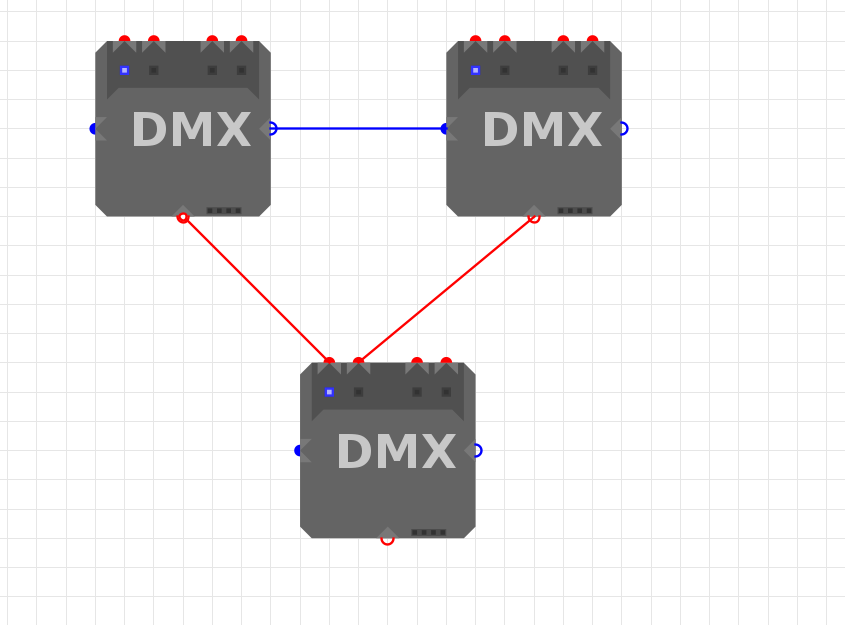
\includegraphics[width =0.57\textwidth]{Images/Screenshot from 2022-12-14 16-31-07.png}
    \caption{Demultplexers}
    \label{fig:demux}
    \end{figure}
\begin{enumerate}
    \item What is the purpose of this circuit ?
    \textcolor{red}{\textbf{Answer:}} One-hot encode the Opcode\\
    \item What is the input the bottom and top demultiplexers ?
    \textcolor{red}{\textbf{Answer:}} Bottom DMX Opcode MSB (2-bit), Top DMX Opcode LSB (2-bit)\\
    \item Which component in Modulesim can provide the desired functionality for (2.)?
       \textcolor{red}{\textbf{Answer:}} Split-Merge\\
\end{enumerate}
\subsubsection{Control Signal}
Different stages of the CPU either derive the same control signal or target the same hardware. \\
\textcolor{red}{\textbf{Answer:}} We use OR blocks\\
\textbf{Question:} What ModuleSim components can you use to implement this functionality ? \\
\textbf{Question:} Consider the following ALU diagram and 4-bit control logic the each of the components:
\begin{figure}[H]
    \centering
    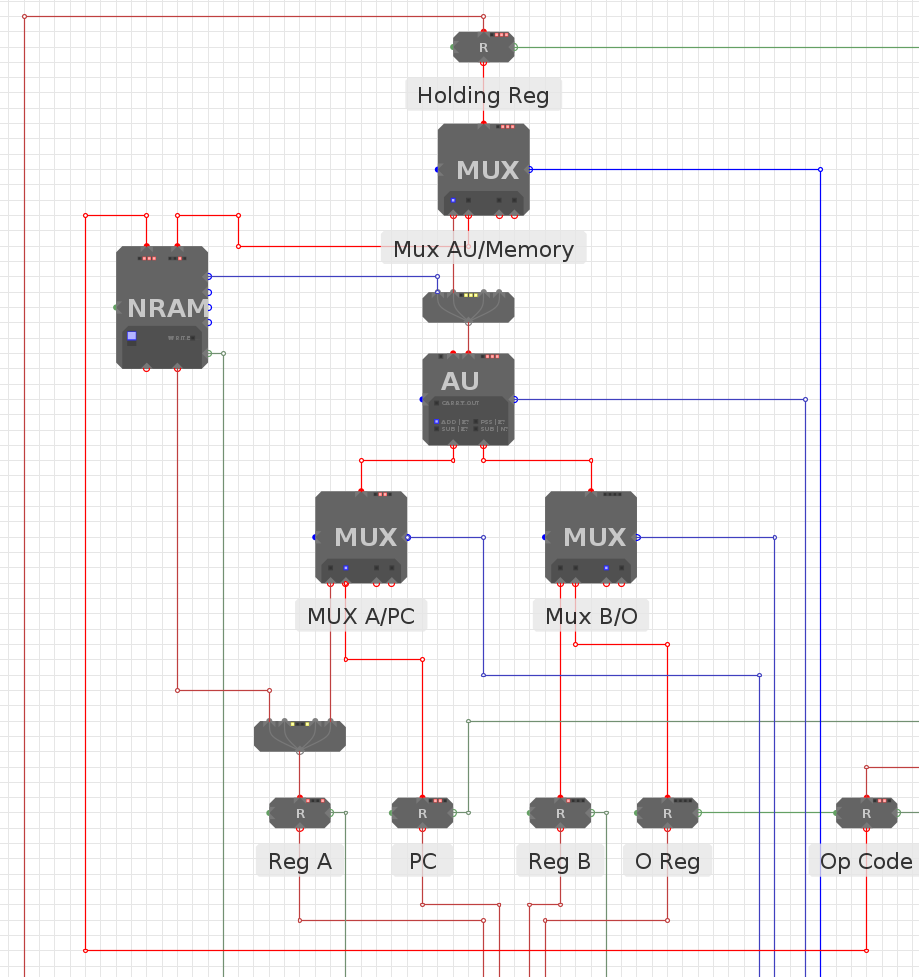
\includegraphics[width =0.57\textwidth]{Images/Screenshot from 2022-12-14 16-40-47.png}
    \caption{ALU}
    \label{fig:demux}
    \end{figure}
\begin{enumerate}
    \item What is the input to the AU/Memory MUX in phase 1  ? \\
     \textcolor{red}{\textbf{Answer:}} 0001 to select the NRAM data\\
    \item Which register(s) are "enabled" in phase 1.b ? \\
    \textcolor{red}{\textbf{Answer:}} O Reg, Opcode Reg\\
    \item What are the inputs to MUX A/PC and B/O in phase 2 ? \\
    \textcolor{red}{\textbf{Answer:}} 0001 for MUX A/PC to select the PC and 0010 for MUX B/O to select a '0' so we can perform PC + 0 + Carry (the correct input need to be set to AU)\\
    \item Describe the process of implementing the STAM instructions. (i.e. Dataflow and control signal)
    \textcolor{red}{\textbf{Answer:}} 
    The first step is to fetch the instruction  (Refer to the  xlsx file) \\
    Then we need to incrememt PC+1 \\
    Decode the instuction using our DMX system\\
\end{enumerate}
%#\bibliographystyle{alpha}
%\bibliography{sample}

\end{document}